\documentclass[a4paper,12pt]{amsart}
\usepackage[T1, T2A]{fontenc}

\usepackage[utf8]{inputenc}
\usepackage{multirow}

\usepackage{amsmath}
\usepackage{amsthm}
\usepackage{relsize}
\usepackage{graphicx}
\usepackage{amssymb,stackengine}

%\usepackage[english]{babel}
\usepackage[ukrainian, english]{babel}

\usepackage{listings}
% \usepackage[colorlinks]{hyperref}
\usepackage{hyperref}
\usepackage[title]{appendix}


% template
\frenchspacing \righthyphenmin=2 \emergencystretch=5pt
\hfuzz=0.5pt \tolerance=400 \oddsidemargin 5mm \evensidemargin 5mm
\textwidth 160mm \textheight 230mm

\hoffset=-0.5cm \voffset=-1.0cm

%\renewcommand\baselinestretch{1.1}



\usepackage{xcolor}

% links
\hypersetup{
	colorlinks=true,
	linkcolor=blue,
	filecolor=magenta,
	urlcolor=cyan,
}

% coloring of listings


\definecolor{codegreen}{rgb}{0,0.7,0}
\definecolor{codegray}{rgb}{0.4,0.4,0.4}
\definecolor{codepurple}{rgb}{0.58,0,0.82}
\definecolor{backcolour}{rgb}{0.95,0.95,0.92}

\lstdefinestyle{mystyle}{
	backgroundcolor=\color{backcolour},
	commentstyle=\color{codegray}\textit,
	keywordstyle=\color{magenta},
	numberstyle=\tiny\color{codegray},
	stringstyle=\color{codepurple},
	%	basicstyle=\ttfamily\footnotesize,
	breakatwhitespace=false,
	breaklines=true,
	captionpos=b,
	keepspaces=true,
	numbers=left,
	numbersep=3pt,
	showspaces=false,
	showstringspaces=false,
	showtabs=false,
	tabsize=2
}

\lstset{style=mystyle}


% path to images
\graphicspath{ {../../graphs/} }

\usepackage[left=2.5cm,right=3cm,
top=2cm,bottom=2cm,bindingoffset=0cm]{geometry}

\title{ 	Складність проблеми слів в Ханойських групах }
\author{ David Zashkolny }
\date{March 2020}

\newtheorem{definition}{Definition}
\newtheorem{corollary}{Corollary}
\newtheorem{hypothesis}{Conjecture}
\newtheorem{proposition}{Proposition}

\newtheorem{theorem}{Theorem}
\newtheorem{lemma}{Lemma}


\begin{document}
	
	
	\thispagestyle {empty}
	\begin{center}
		\large  Київський Національний Університет імені Тараса Шевченка \\
		Механіко-математичний факультет \\
		Кафедра алгебри і комп'ютерної математики \par
	\end{center}
	
	
	\begin{center}
		\vskip0cm plus 2fill
		\vspace{2.5cm} {\bf Курсовий проект}\\
		
		%{\bf на здобуття ступеня магістра математики}\\
		{\bf на тему:}\\
	\end{center}
	
	
	\vskip0cm plus 1.0fill
	
	
	
	\begin{center}\bf
		{\LARGE
			Self-similar actions of the wallpaper groups 
		\par}
	\end{center}
	
	\vskip0cm plus 1.5fill
	
	\hangindent=7cm \hangafter=0 \noindent
	Виконав\\
	студент 1-го курсу магістратури\\
	напрям математика\\
	спеціалізація "комп'ютерна математика"\\
	{\bf Зашкольний Давид Олександрович}\\[2cm]
	Науковий Керівник:\\
	Доцент кафедри, доктор фiзико-математичних наук\\
	{\bf Бондаренко Євген Володимирович}
	
	
	\vskip0cm plus 1.5fill
	
	\vskip5cm plus 1.5fill
	\begin{center}
		КИЇВ --- 2022
	\end{center}
	
	\newpage
	\pagenumbering{arabic}
	
	%\newpage
	\tableofcontents
	
	\newpage
	
	\section{Introduction}
	This article is focused on the crystallographic groups as discrete groups of motions of an $n$-dimensional Euclidean space having a bounded fundamental domain. Particularly on the existence of faithful self-similar action in case of $n=2$ using results of Volodymyr Nekrashevych \cite{Nekrashevych} (proposition 2.9.2). We examined every crystallographic group in $R^2$ whether they have such action in order to develop the criterion in general case. The results are illustrated in Table \ref{tab:self-similar} and \ref{tab:normalizers}. Those, along with code, also can be found on the GitHub \href{https://github.com/davendiy/master_thesis}{repository}.
	
	
	\section{Prerequisites}
	
	In this section we define all the constructions which we will need for studying the main topic.
	
	\subsection{Rooted trees}
	
	Let X be a finite set, which we call \textit{alphabet}. By $X^*$ we denote the set 
	
	$$\{x_1 x_2 \dots x_n : x_i \in X \}$$
	
	of all finite words over the alphabet $X$, including an empty word $\emptyset$. Naturally, $X^*$ with the concatenation of words as binary action make the \textit{free monoid} generated by $X$. By $|v|$ we denote the \textit{lengths} of a word $v = x_1 x_2 \dots x_n$
	
	It is a convenient way to think about $X^*$ as a rooted tree, where two vertices are connected by the edge iff the associated words have forms $v$ and $vx$ respectively, where $v \in X^*, x \in X$. Obviously, the empty word $\emptyset$ is the root of the tree.
	
	
	\begin{figure}[h]
		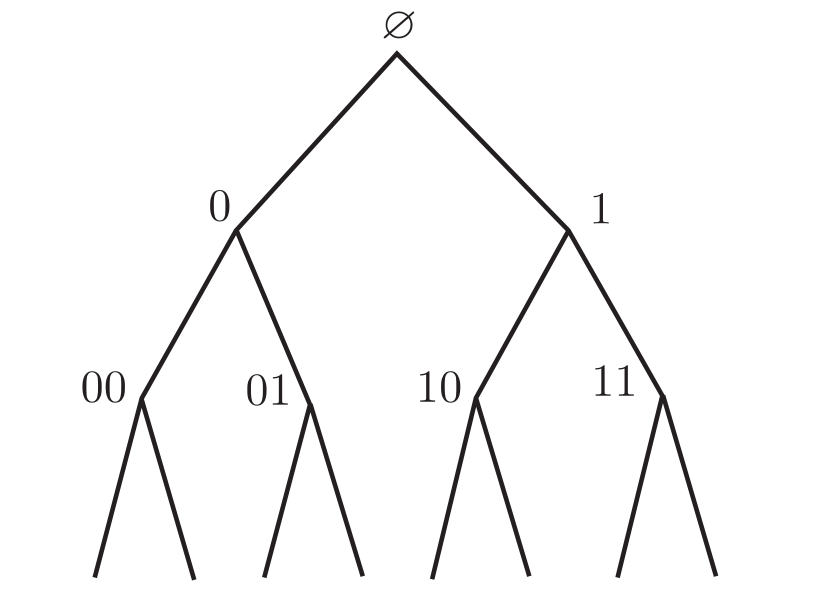
\includegraphics[scale=0.4]{rooted2tree.png}
		\caption{Example of the rooted tree in case of $X = \{0,1\}$}
	\end{figure}
		
	The set $X^n \subset X$ is called the \textit{$n$-th level} of the tree $X^*$. A map $f:X^* \rightarrow X^*$ is an \textit{endomorphism} of the tree $X^*$ if for any adjacent vertices $u, v$ their images $f(u)$ and $f(v)$ are also adjacent. Thus, taking into account the exact form of adjacent vertices in $X^*$, $f(ux) = f(u)y$, where $x, y \in X$.
	
	It is easy to check that $f(X^*) \subset X^*$, which means that we map the entire tree $X^*$ on it's subtree $uX^*$, where $u \in X^*$ is a \textit{prefix}. If $f$ is bijective then it is called an $automorphism$.
	
	In addition, we consider a $X^\omega$ set of all possible infinite-length words over the alphabet $X$ that is the \textit{boundary} of the tree $X^*$. Naturally, the endomorphism $f(x)$ can be extended uniquely upon the $X^* \sqcup X^\omega$.
	
	Denote by $AutX^*$ the group of all automorphisms of the rooted tree $X^*$.
	
	\subsection{Groups actions}
	A group $G$ is (left) acting on a set $X$ if a map $G \times X \rightarrow X, (g, x) \mapsto g(x)$ with following properties is defined: 
	
	\begin{enumerate}
		\item $(gh)(x) = g(h(x))$ for every $g, h \in G, x \in X$
		\item $e(x) = x$ for every $x \in X$, where $e$ is a group's identity.
		 
	\end{enumerate}
		
	In other words, action of $G$ on $X$ means a homomorphism from $G$ to $Sym(X)$. Recall that $AutX^* \subset Sym(X^*)$ since not every bijection of $X^*$ on itself is a homomorphism.
	
	Group action is
	
	\begin{itemize}
		\item[-] \textit{transitive} if $X$ is non-empty and for each pair $x,y \in X$ there exists a $g \in G$ such that $g(x) = y$.
		\item[-] \textit{regular} (or \textit{simply transitive}) if it is transitive and there exists only one $g$ for every pair $x, y$ 
		\item[-] \textit{faithful} if for every $g \neq e \in G$ there exists $x \in X$ such that $g(x) \neq x$
		\item[-] \textit{free} if for every $g \neq e \in G, \, g(x) \neq x$ for every $x \in X$ 
	\end{itemize}
	
	Faithful action means that the homomorphism $G \rightarrow Sym(X)$ induced by the action \textit{has trivial kernel}. 
	
	\begin{proposition}
		Action is regular iff it is both transitive and free. 
	\end{proposition}
	
	\subsection{Automata}
	In general, an \textit{invertible automaton} is a quadruple $A = (S, X, \tau, \pi)$ where $S$ is a finite set of states, $X$ is a finite alphabet, $\tau: S\times X \rightarrow S$ a \textit{transition function} and $\pi : S \times X \rightarrow X$ an \textit{output function} such that, for each state $s \in S$, the restriction $\pi_s = \pi(s) : X \rightarrow X$ is a permutation in $S_X$ (see \cite{Auto}).  If, for instance, the automaton is complete and invertible then its states generate a group, also known as \textit{automaton group}. 
	
	\subsection{Self-similar actions}
	Let $g : X^* \rightarrow X^* $ be an endomorphism of the rooted tree $X^*$. Consider a vertex $v \in X^*$ and $vX^*$ along with $g(v)X^*$ -- subtrees of $X^*$ with $v$ and $g(v)$ as the root respectfully. $vX^*$ represents all the words from $X^*$ that start with $v$ as the prefix. Then, consider a map $g\arrowvert_v: vX^* \rightarrow g(v)X^*$ that is a \textbf{restriction} of the $g$ on $v$. The subtree $vX^*$ is naturally isomorphic to the entire $X^*$ via the map $vw \mapsto w$, as well as $g(v)X^*$. Therefore,
	
	\begin{proposition}
		$g\arrowvert_v$ is an \textit{endomorphism} of $vX^*$ and $g(v)X^*$. It is uniquely determined by the condition 
	
		$$g(vw) = g(v)g\arrowvert_v(w)$$
	 
	\end{proposition}
	 
	\begin{figure}[h]
	 	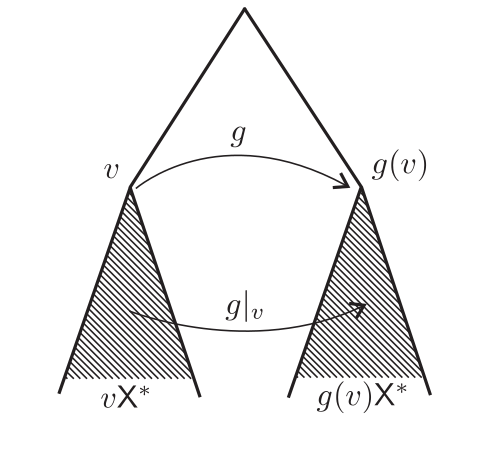
\includegraphics[scale=0.8]{restriction.png}
	 	\caption{Restriction $g\arrowvert_v$}
	 \end{figure}
	 
	 Here are the obvious properies of the restrictions: 
	 
	 $$g\arrowvert_{v_1v_2} = g\arrowvert_{v_1}\arrowvert_{v_2}$$
	 $$(g_1 \cdot g_2)\arrowvert_v = g_1\arrowvert_v \cdot g_2\arrowvert_v$$
	 
	 Now let's define one of the main properties for this article. 
	 
	\begin{definition}\label{def:self_similar_action}
		A faithful action of a group $G$ on $X^*$ (or on $X^\omega$) is said to be \textbf{self-similar} if for every $g \in G$ and every $x \in X$ there exist $h \in G$ and $y \in X$ such that 
		
		$$g(xw) = yh(w)$$
		
		for every $w \in X^*$ ($w \in X^\omega$ resp.)
	\end{definition}

	We will denote 	self-similar actions as pairs $(G, X)$, where $G$ is the group and $X$ is the alphabet (meaning that $G$ acts on $X^*$ or $X^\omega$).
	
	The pair $(h, y)$ is uniquely determined in the conditions of the Definition \ref{def:self_similar_action} by the pair $(g, x)$ since the action is faithful. Hence, we get an automaton with the set of stages $G$ and with the output and transition functions
	
	$$g \cdot x = y \cdot h$$
	
	where $y = g(x)$ and $h = g\arrowvert_x$. Hereby, any element $g \in G$ can be defined accordingly to it's action on $X^*$: 
	
	$$g = \pi (g\arrowvert_{x_1} g\arrowvert_{x_2} \dots g\arrowvert_{x_n})$$
	
	where $\pi \in Sym(X)$, such that $\pi(x) = y$ from the previous thesis, $X = \{x_1 x_2 \dots x_n\}$. This notation is also called \textit{wreath recursion}, that is a homomorphism 
	
	$$\phi : G \rightarrow Sym(X) \wr G$$
	
	and the symbol $\wr$ is a \textit{wreath product}, however in this article we will not use any properties of this operation. One can found more details in \cite{Nekrashevych}.
	
	
	
	
	The next definition is equivalent to \ref{def:self_similar_action} but emphasizes the relation with automata. 
	
	\begin{definition}
		A faithful action of a group $G$ on $X^*$ is said to be \textbf{self-similar} if there exists an automaton $(G, X)$ such that the action of $g \in G$ on $X^*$ coincides with the action of the stage $g$ of the automaton. 
	\end{definition} 

	Since $G$ acts on $X^*$ faithfully, then $G$ is isomorphic to a subgroup of the $Aut X^*$. Therefore, the definition \ref{def:self_similar_action} can also be formulated in term of rooted trees: 
	
	\begin{definition}
		An automorphism group $G$ of the rooted tree $X^*$ is \textbf{self-similar} if for every $g \in G$ and $v \in X^*$ we have $g\arrowvert_v \in G$.
	\end{definition} 
	
	
	An important class of self-similar actions are \textit{contracting} actions, that is there exists a finite set $\mathcal{N}$ such that for every $g \in G$ there exists $k \in \mathbb{N}$ such that $g\arrowvert_v \in \mathcal{N}$ for all words $v \in X^*$ of length $\ge k$. The smallest set $\mathcal{N}$ with this property is called the \textit{nucleus} of the self-similar action. 
	
	\subsection{Crystallographic groups}
	
	Let $\mathbb{R}^n$ be an $n$-dimensional Euclidean space with the standard scalar product $\langle.\rangle$, euclidean norm $||.||$ and the metric induced by it $d(., .)$. A map $f : \mathbb{R}^n \rightarrow \mathbb{R}^n$ shall be called an \textit{isometry} if for any $x, y \in \mathbb{R}^n$
	
	$$d(x, y) = d(f(x), f(y)).$$
	
	It is easy to prove, that the set of all isometries of $\mathbb{R}^n$ is a group with respect to composition of maps. Hereby $E(n)$ shall denote the group of all isometries of the Euclidean space $\mathbb{R}^n$. 
	
	Any isometry of the space $\mathbb{R}^n$ is a composition of an orthogonal linear map and a translation, i.e. if $f : \mathbb{R}^n \rightarrow \mathbb{R}^n$ is an isometry of $\mathbb{R}^n$, then there exist a translation $t_a$ and an orthogonal map $A: \mathbb{R}^n \rightarrow \mathbb{R}^n$ such that $f = A \circ t_a$ . That means for every $x \in \mathbb{R}^n$
	
	$$f(x) = Ax + a$$ 
	
	where $A$ is an orthogonal matrix. The group of all orthogonal operators is denoted by $O(e)$, whilst the group of all translations is isomorphic to the $\mathbb{R}^n$.
	
	Now, let's introduce a useful construction
	
	\begin{definition}
		Let $H$ and $K$ denote groups with multiplication '$\circ$' and '$\star$' respectively. Moreover, assume that H is a subgroup of the authomorphism group $Aut K$ of the abelian group $K$. The \textbf{semi-direct} product $H \ltimes K$ of the groups $H$ and $K$ is the set of pairs $(h, k)$ with the following multiplication
		
		$$(h_1, k_1)(h_2, k_2) = (h_1 \circ h_2, k_1 \star h_1 (k_2))$$
	\end{definition}
	
	The multiplication from the previous definition is, in fact, multiplication in the affine group $A(n)$ 
	
	$$A(n) = GL(n, \mathbb{R}) \ltimes \mathbb{R}^n$$
	
	and, in our case, the group of isometries 
	
	$$E(n) = O(n) \ltimes \mathbb{R}^n$$
	
	
	\begin{proposition}
		There is following sequence of subgroups: 
		
		$$E(n) \subset A(n) \subset GL(n + 1, \mathbb{R})$$
	\end{proposition}

	\begin{definition}
		Let $X$ be a metric space and $\Gamma$ a subgroup of a group of its isometries. An open, connected subset $F \subset X$ is a \textbf{fundamental domain} if 
		
		$$X = \bigcup_{g \in G} g \bar{F}$$
		
		and $gF \cap g'F = \emptyset$, for $g \ne g' \in G$
	\end{definition}

	
	\begin{definition}
		A \textbf{crystallographic} group of dimension $n$ is a cocompact and discrete subgroup of $E(n)$.
	\end{definition}

	\begin{theorem}
		(Bieberbach) 
		
		1. If $\Gamma \subset E(n)$ is a crystallographic group then the set of translations $\Gamma \cap (I \times \mathbb{R}^n)$ is a torsion free and finitely generated abelian group of rank $n$, and is a maximal abelian and normal subgroup of finite index. 
		
		2. For any natural number $n$, there are only a finite number of isomorphism classes of crystallographic groups of dimension $n$.
		
		3. Two crystallographic groups of dimension $n$ are isomorphic if and only if they are conjugate in the group $A(n).$
	\end{theorem}

	
	\begin{proposition}
		Properties of crystallographic groups: 
		
		- If $\Gamma$ is an abelian crystallographic group; then $\Gamma$ contains only pure translations. 
		
		- (Zassenhaus theorem) A group $\Gamma$ is isomorphic to a crystallographic group of dimension $n$ iff $\Gamma$ has a normal, free abelian subgroup $\mathbb{Z}^n$ of finite index which is a maximal abelian subgroup of $\Gamma$.	
	
        
	\end{proposition}

	\newpage
	\section{Problem}
	
	\subsection{Self-similar actions of $\mathbb{Z}^n$}
	
	Consider a self-similar action $(G, X)$.
	
	\begin{definition}
		The map $\phi_x : G_x \rightarrow G$ defined by the formula 
		
		$$\phi_x(g) = g\arrowvert_x$$
		
		is a virtual endomorphism of $G$. Here $G_x$ is the stabilizer of the one-letter word $x$ in $G$. The $\phi : G \dashrightarrow G$ is called the \textbf{endomorphism associated to the self-similar action}. 
	\end{definition}
	
	\begin{proposition}
		The kernel of a self-similar action of a group $G$ with an associated virtual endomorphism $\phi$ is equal to the subgroup 
		
		$$K(\phi) = \bigcap_{n\ge 1}\bigcap_{g \in G} g^{-1} \cdot Dom \phi^n \cdot g$$
		
		and is the maximal one among the normal $\phi$-invariant subgroups.
	\end{proposition}
	
	\begin{corollary}
		If $G$ is an abelian group, then the kernel of a self-similar action  is equal to the subgroup 
		$$K(\phi) = \bigcap_{n\ge 1} \phi^{-n}(G)$$
		
	\end{corollary}
	
	Now, consider such an action $G = \mathbb{Z}^n$ and let $\phi : \mathbb{Z}^n \dashrightarrow \mathbb{Z}^n$ be the associated virtual endomorphism. $\phi$ can be uniquely extended to a linear map $A : \mathbb{Q}^n \rightarrow \mathbb{Q}^n$.
	
	Hereby $A$ shall also denote the matrix of the linear operator $A$ in the standard basis. The matrix $A$ obviously has rational entries and moreover $k \cdot A$ contains only integers, where $k \in \mathbb{N}$ is such that $k\mathbb{Z}^n \le Dom \phi$.
	
	If $\phi$ is a surjection and invertible, then the map $\phi^{-1}$ is injective and defined on the entire $\mathbb{Z}^n$. Thus and so $A^{-1}$ is a matrix of integers.
	
	Let $T = \{g_i,\, i=1..k\}$ be a coset transversal of the $Dom \phi$ and $X = \{x_i,\, i=1..k\}$.	
	
	\begin{proposition}
		The self-similar action (not necessary faithful) of $G$ on $X$, that is defined in the following way 
		
		$$g \cdot x_i = x_j \cdot \phi(g_j^{-1} g g_i)$$
		
		where $j$ is such that $g^{-1}_j g g_i \in Dom \phi $. 
	\end{proposition}
	
	The defined self-similar action is faithful iff its kernel is trivial. Due to \cite{Nekrashevych} we have a criterion
	
	\begin{theorem}(Nekrashevych) \label{theorem:Nekrashevych}
		The subgroup $K(\phi)$ is trivial if and only if characteristic polynomial
		of $A$ is not divisible by a monic polynomial with integral coefficients (or, in other words, if and only if no eigenvalue of A is an algebraic integer)
	\end{theorem}
	
	
	\subsection{Crystallographic case}
	
	Now instead of $\mathbb{Z}^n$ consider a crystallographic group $\Gamma \subset E(n)$. Recall that, since $E(n) = O(n) \ltimes \mathbb{R}^n$, every element $g \in \Gamma$ has a form 
	
	$$g(x) = a(x) + t,$$ 
	where $a$ is a \textit{linear part} and $t$ is a \textit{translation}. Along with $\Gamma$ we will consider a group $G$ (sometimes referred to as a \textit{Point Group}) of all the linear parts of $\Gamma$ and the set $L$ of all parallel translations in $\Gamma$. Recall that $L$ is in fact a normal subgroup of finite index, isomorphic to $\mathbb{Z}^n$. Since $G$ preserves the lattice $L$, relative to a basis in $L$ the transformations in $G$ are represented by matrices with integer entries. 
	
	However, it is clear that not every pair $(g, t), \, g \in G, \, t \in L$ can appear in the $\Gamma$. Thus, in order to specify the $\Gamma$, we further have to provide a map $a(g)$ such that 
	
	$$x \mapsto g x + a(g), \, x \in \mathbb{R}^n$$
	
	It should be also mentioned, that a mapping 
	
	$$\alpha : g \mapsto a(g) + L$$
	
	is in fact a one-dimensional cohomologous cocycle, and any crystallographic group can be represented as a triplet $(G, L, \alpha)$, but for the sake of sancta simplicitas we won't use it here. 
	
	The central problem of this article is the following: \textbf{\textit{which crystallographic groups admit the self-similar action?}}. 
	
	Keeping in mind the afore-described approach for $\mathbb{Z}^n$, firstly we have to build a virtual endomorphism of $\Gamma$. Recall that by the Bieberbach theorem two crystallographic groups $\Gamma_1$ and $\Gamma_2$ are isomorphic if and only if they are conjugate in the group $A(n)$, or in other words there exists $a \in A(n)$ such that 
	
	$$\Gamma_1 = a^{-1} \Gamma_2 a$$
	
	which gives us a natural way to define the virtual endomorphism $\phi : \Gamma \dashrightarrow \Gamma$: 
	
	$$\phi_a(g) = a^{-1} g a$$.
	
	Now, rewrite this equation taking into account $a = g_{(A, v)}, \, g = g_{(O, t)}$:
	
	$$\phi_a (g_{(O, t)}) = g^{-1}_{(A, v)} \cdot g_{(O, t)} \cdot g_{(A, v)} = g^{-1}_{(A, v)} \cdot g_{(OA, Ov + t)} = g^{-1}_{(A^{-1}, -A^{-1}v)} \cdot g_{(OA, Ov + t)} $$
	
	\begin{equation}
		\label{eq:eq1}
		\phi_a (g_{(O, t)}) = g_{(A^{-1}OA, \, A^{-1}(Ov + t - v))}
	\end{equation}
	
	Here we see, that the linear part $G$ should be invariant with respect to conjugation by $A$ in order to make $\phi$ to be the endomorphism indeed. In other words, $A$ should belong to a normalizer of $G$.
	
	Considering the case when $O = \mathbb{I}_n$
	
	\begin{equation}
		\label{eq:eq1}
		\phi (g_{(\mathbb{I}_n, t)}) = g_{(\mathbb{I}_n, \, A^{-1}t)}
	\end{equation}
		
	
	it is clear that $A$ is also "accountable" for the endomorphism on transitions $L$. Hence, we have the following.
	
	\begin{proposition}
		If $\phi_{a}$ is an associated virtual endomorphism of a faithful self-similar action $\Gamma, X$, where $a = g_{(A, v)}$, then $A$ should satisfy the Nekrashevych condition from Theorem \ref{theorem:Nekrashevych}.
	\end{proposition}
	
	
	\newpage 
	\section{Experiments}
	Having a theoretical toolkit from the previous section, we investigated all the planar (i.e. two-dimensional) crystallographic groups whether they admit the faithful self-similar action or not. Up to equivalence, there are 17 planar crystallographic groups (\cite{Fedorov}, \cite{Schoenflies}), yet amount of unique Point Groups is only 11.
	
	On the Table \ref{tab:self-similar} we present all the associated virtual endomorphisms for the planar crystallographic groups, which were found applying the aforementioned approach. 
	

	
	\begin{table}[h]
		\begin{tabular}{|c|c|c|c|c|}
			\hline
			№ & \textbf{Generators} &  \textbf{$\phi$} & \textbf{|X|} & Exact form \\
			\hline 
			
			
			1 & \multirow{2}{*}{$\left\langle 
					\begin{pmatrix}
						1 & 0 \\ 
						0 & 1 
					\end{pmatrix} 			
				\right\rangle$
			}
			   & \multirow{2}{*}{$\left(\begin{array}{cc|c}
			   	0 & 2 & 0\\ 
			   	1 & 0  & 0
			\end{array}\right)$  
		   	}
		   	   & \multirow{2}{*}{2} & $a = () (b, b) $\\
		   	   
		   	   &  & & & $b = (12)(a, e)$      \\
		   
		   \multirow{3}{*}{2} & \multirow{3}{*}{$\left\langle 
		   	\begin{pmatrix}
		   		-1 & 0 \\ 
		   		0 & -1 
		   	\end{pmatrix} 			
		   	\right\rangle$
		   }
		   	& \multirow{3}{*}{$\left(\begin{array}{cc|c}
		   		0 & 2  & 0\\ 
		   		1 & 0  & 0
		   	\end{array}\right)$  
		   }
		   	& \multirow{3}{*}{2} & $a = () (b, b)$\\
		   	& & & & $b = (12)(a, e)$\\
		   	& & & & $c = ()(c, ca^{-1})$\\
		   	
		   3 & $\left\langle 
		   	\begin{pmatrix}
		   		-1 & 0 \\ 
		   		0 & 1 
		   	\end{pmatrix} 			
		   	\right\rangle$
		   	
		   	& -
		   	& - & \\
		   	
		  4 & $\left\langle 
		   \left(\begin{array}{cc|c}
		   	-1 & 0  & 0 \\ 
		   	0 & 1   & \frac{1}{2}
		  \end{array}\right) 			
		   \right\rangle$
		   
		   & -
		   & -  & \\	
		  
		  5 & $\left\langle 
		  \begin{pmatrix}
		  	-1 & 0  \\ 
		  	0 & 1  
		  \end{pmatrix}, 
	   	\begin{pmatrix}
	   		\frac{1}{2} \\ 
	   		\frac{1}{2}  
	   	\end{pmatrix}		
		  \right\rangle$
		  
		  & -
		  & - & \\	
		  
		  \multirow{4}{*}{6} & \multirow{4}{*}{$\left\langle 
		  \begin{pmatrix}
		  	-1 & 0  \\ 
		  	0 & -1  
		  \end{pmatrix},
		  \begin{pmatrix}
		  	-1 & 0  \\ 
		  	0 & 1  
		  \end{pmatrix}  	
		  \right\rangle$
		  }
		  & \multirow{4}{*}{$\left(\begin{array}{cc|c}
		  	0 & 2  & 0\\ 
		  	1 & 0  & 0
		\end{array}\right)$ } 
		  & \multirow{4}{*}{2} & $a = () (a, ac^{-1})$ \\	
		  
		  & & & & $b = () (ba, ba)$\\
		  & & & & $c = () (d, d)$\\
		  & & & & $d = (1 2) (c, e)$\\
		  
		  
		   7 & $\left\langle 
		  \begin{pmatrix}
		  	-1 & 0  \\ 
		  	0 & -1  
		  \end{pmatrix}, 
		  \left(\begin{array}{cc|c}
		  	-1 & 0 & \frac{1}{2} \\ 
		  	 0 & 1 & 0  
		  \end{array}\right)		
		  \right\rangle$
		  
		  & -
		  & - &\\	
		  
		  
		  \multirow{4}{*}{8} & \multirow{4}{*}{$\left\langle 
		  \begin{pmatrix}
		  	-1 & 0  \\ 
		  	0 & -1  
		  \end{pmatrix}, 
		  \begin{pmatrix}
		  	\frac{1}{2} \\ 
		  	\frac{1}{2}  
		  \end{pmatrix}		
		  \right\rangle$
		}
		  & \multirow{4}{*}{$\left(\begin{array}{cc|c}
		  	0 & 3  & 0\\ 
		  	1 & 0  & 0
		\end{array}\right)$ }
		  & \multirow{4}{*}{3} &  $a = (2 3) (a, b c^{-1} d^{-1}, bc^{-1})$\\
		  
		  & & & & $b = (1 3 2) (bacd, e, e)$ \\
		  & & & & $c = (3) (d, d^{-1}, d)$ \\
		  & & & & $d = (1 2 3) (bacd, bacd, e)$ \\
		  
		  9	 & $\left\langle 
		  \begin{pmatrix}
		  	-1 & 0  \\ 
		  	0 & -1  
		  \end{pmatrix}, 
		  \begin{pmatrix}
		  	-1 & 0  \\ 
		  	0 & 1  
		  \end{pmatrix},
		  \begin{pmatrix}
		  	\frac{1}{2} \\ 
		  	\frac{1}{2}  
		  \end{pmatrix}		
		  \right\rangle$
		  
		  & $\left(\begin{array}{cc|c}
		  	0 & 3  & 0\\ 
		  	1 & 0  & 0
		\end{array}\right)$ 
		  & 3 &\\
		  
		  
		  10 & $\left\langle 
		  \begin{pmatrix}
		  	-1 & 0  \\ 
		  	0 & -1  
		  \end{pmatrix}, 
		  \begin{pmatrix}
		  	0 & 1  \\ 
		  	-1 & 0  
		  \end{pmatrix}
		  \right\rangle$
		  
		  & $\left(\begin{array}{cc|c}
		  	1 & -1  & 0\\ 
		  	1 & 1  & 0
		\end{array}\right)$ 
		  & 2 &\\
		  
		  11 & $\left\langle 
		  \begin{pmatrix}
		  	-1 & 0  \\ 
		  	0 & -1  
		  \end{pmatrix}, 
		  \begin{pmatrix}
		  	0 & 1  \\ 
		  	-1 & 0  
		  \end{pmatrix}
		  \begin{pmatrix}
		  	-1 & 0  \\ 
		  	0 & 1  
		  \end{pmatrix}
		  \right\rangle$
		  
		  & $\left(\begin{array}{cc|c}
		  	1 & -1  & 0\\ 
		  	1 & 1  & 0
		\end{array}\right)$ 
		  & 2 &\\
		  
		  
		  12 & $\left\langle 
		  \begin{pmatrix}
		  	-1 & 0  \\ 
		  	0 & -1  
		  \end{pmatrix}, 
		  \begin{pmatrix}
		  	0 & 1  \\ 
		  	-1 & 0  
		  \end{pmatrix}
		  \left(\begin{array}{cc|c}
		  	-1 & 0 &  \frac{1}{2} \\ 
		  	0 & 1  & \frac{1}{2}
		\end{array}\right)
		  \right\rangle$
		  
		  & $\left(\begin{array}{cc|c}  
		  	0 & -3  & 0\\ 
		  	3 & 0  & 0
		  	\end{array}\right)$ 
		  & 9 &\\
		  
		   13 & $\left\langle 
		  \begin{pmatrix}
		  	0 & 1 \\ 
		  	-1 & -1 
		  \end{pmatrix} 			
		  \right\rangle$
		  
		  & $\left(\begin{array}{cc|c}  
		  	1 & -1  & 0\\ 
		  	1 & 2   & 0
		\end{array}\right)$  
		  
		  & 3 &\\
		  
		  
		   14 & $\left\langle 
		  \begin{pmatrix}
		  	0 & 1 \\ 
		  	-1 & -1 
		  \end{pmatrix}, 			
		  \begin{pmatrix}
		  	0 & -1 \\ 
		  	-1 & 0
		  \end{pmatrix}
		  \right\rangle$
		  
		  & $\left(\begin{array}{cc|c}  
		  	2 & 2  & 0\\ 
		  	-2 & 0   & 0
		  \end{array}\right)$  
		  
		  & 4 &\\
		  
		   15 & $\left\langle 
		  \begin{pmatrix}
		  	0 & 1 \\ 
		  	-1 & -1 
		  \end{pmatrix}, 			
		  \begin{pmatrix}
		  	0 & 1 \\ 
		  	1 & 0
		  \end{pmatrix}
		  \right\rangle$
		  
		  & $\left(\begin{array}{cc|c}  
		  	2 & 2  & 0\\ 
		  	-2 & 0   & 0
		  \end{array}\right)$  
		  
		  & 4 &\\
		  
		   16 & $\left\langle 
		  \begin{pmatrix}
		  	0 & 1 \\ 
		  	-1 & -1 
		  \end{pmatrix}, 			
		  \begin{pmatrix}
		  	-1 & 0 \\ 
		  	0 & -1
		  \end{pmatrix}
		  \right\rangle$
		  
		  & $\left(\begin{array}{cc|c}  
		  	1 & -1  & 0\\ 
		  	1 & 2   & 0
		  \end{array}\right)$  
		  
		  & 3 &\\
		  
		  17 & $\left\langle 
		  \begin{pmatrix}
		  	0 & 1 \\ 
		  	-1 & -1 
		  \end{pmatrix}, 			
		  \begin{pmatrix}
		  	-1 & 0 \\ 
		  	0 & -1
		  \end{pmatrix},
		  \begin{pmatrix}
		  	0 & -1 \\ 
		  	-1 & 0
		  \end{pmatrix}
		  \right\rangle$
		  
		  & $\left(\begin{array}{cc|c}  
		  	2 & 2  & 0\\ 
		  	-2 & 0   & 0
		  \end{array}\right)$  
		  
		  & 4 &\\
		  
		  \hline
		\end{tabular}
	
	\caption{Faithful self-similar actions in the planar crystallographic groups, defined by the associated virtual endomorphism}
	
	\label{tab:self-similar}
	\end{table}
	
	Some 'notate bene' relating to the table \ref{tab:self-similar}: column "generators" skips the default translations (those are $\begin{pmatrix}1 \\ 0\end{pmatrix}$ and $\begin{pmatrix}0 \\ 1\end{pmatrix}$); zero translations along with unitary matrices are skipped as well; $|X|$ means the size of the alphabet that is the transversal of $\Gamma / \phi(\Gamma)$ (hypothetically, it equals to the determinant of the endomorphism matrix); exact form of the self-similar actions is found in every case, although most of them are huge and ugly.  
	
	Table \ref{tab:normalizers} (see appendix) contains normalizers for every point group in $\mathbb{R}$ (i.e. linear part of the given crystallographic group). It was constructed in semi-automatic way using the following technique. 
	
	Consider any point group $G$. By definition, its normalizer $\mathcal{N}$ is the maximal subset of $GL(n, Q)$ that is 
	
	$$\mathcal{N}G = G\mathcal{N}$$.
	
	Thus, let $N = \begin{pmatrix}a & b \\ c & d \end{pmatrix}$. For every possible permutation $\pi \in Sym(G)$ we get a system of linear equations: 
	
	\begin{equation} \label{eq:eq2}
		Ng_i = g_{\pi(i)}N
	\end{equation}
	
	that can be solved using Gaussian elimination for example. Then, denoting the set of solutions as $\mathcal{N}_\pi$ we have
	
	$$\mathcal{N} = \bigcup_{\pi \in Sym(G)}\mathcal{N}_\pi$$.
	
	Fortunately, $G$ are small in the most cases, since for $|G| > 6$ this problem becomes computationally hard. We can reduce the computational space, using an observation that conjugate elements should have the same order. 
	
	
	\begin{proposition} \label{prop:1}
		Crystallographic groups 3, 4, 5 and 7 don't admit self-similar action. 
	\end{proposition}	

	\begin{proof}
		Due to the Table \ref{tab:normalizers}, we see that the normalizer for the groups 3, 4 and 5 contains only diagonal matrices that don't satisfy Nekrashevych condition from theorem \ref{theorem:Nekrashevych}. 
		
		Nevertheless, the 7-th crystallographic group $\Gamma_7$ has the same linear part as the 6-th, where the self-similar action can be constructed. However, considering $A = \left(\begin{array}{cc|c}
			0 & a & x \\ 
			b & 0 & y
		\end{array}\right)$ and $g_2 = \left(\begin{array}{cc|c}
		-1 & 0 & \frac{1}{2} \\ 
		0 & 1 & 0 
	\end{array}\right)$

	$$A^{-1} g_2 A = 
	\left(\begin{array}{cc|c}
		1 & 0 & 0 \\ 
		0 & -1 & \frac{1}{2} a ( \frac{2y}{a}+ 1) + y
	\end{array}\right) \notin \Gamma_7$$

	\end{proof}
	
	\section{Further research}
	
	The main next step to be done is to construct a criterion of crystallographic group admitting self-similar action for the general case $\Gamma < E(n)$. As we could see in the proof of proposition \ref{prop:1}  for potential $A$ it is not enough to satisfy the Nekrashevych condition and belong to normalizer of $G$ for construction a virtual endomorphism $\phi_A$. 
		
	\newpage 
	\begin{thebibliography}{9}
		
		\bibitem{Nekrashevych} "Self-Similar Groups" Volodymyr Nekrashevych,
		International University Bremen, School of Engineering and Sci-
		ence, P.O. Box 750 561, 28725 Bremen, Germany
		
		\bibitem{Cryst_and_math}
		FARKAS, DANIEL R. “CRYSTALLOGRAPHIC GROUPS AND THEIR MATHEMATICS.” The Rocky Mountain Journal of Mathematics, vol. 11, no. 4, 1981, pp. 511–51. JSTOR, http://www.jstor.org/stable/44236620. Accessed 4 Jun. 2022.
		
		\bibitem{Auto}
		R.I. Grigorchuk, V.V. Nekrashevich, V.I. Sushchanskiı, Automata, dynamical systems, and groups, Tr. Mat. Inst. Steklova 231 (2000) 134-214
		(Din. Sist., Avtom. i Beskon. Gruppy).
		
		\bibitem{Fedorov}  	E.S. Fedorov, "The symmetry and structure of crystals. Fundamental works" , Moscow (1949) pp. 111–255
		
		\bibitem{Schoenflies} A. Schoenflies, "Kristallsysteme und Kristallstruktur" , Teubner (1891)
		
	\end{thebibliography}
	
	
	\newpage
	\section{Appendix}
	
	
	\begin{table}[h]
		\begin{tabular}{|c|c|c|c|c|}
			\hline
			
			
			№ & \textbf{Point Group} &  \textbf{Normalizer} & \textbf{Det.} & \textbf{Charpoly} \\ 
			\hline
			
			
			1  & $\left\langle 
					\begin{pmatrix}
						1 & 0 \\ 
						0 & 1 
					\end{pmatrix}
				\right\rangle$			 
			   & $\begin{pmatrix}
			   	a & 0 \\ 
			   	0 & a 
			   \end{pmatrix}$ 
		   		& $a^2$ &  $(a - x)^2$   \\
			   
			2 & $\left\langle 
			\begin{pmatrix}
				-1 & 0 \\ 
				0 & -1 
			\end{pmatrix}
			\right\rangle$			 
			& $\begin{pmatrix}
				a & 0 \\ 
				0 & a 
			\end{pmatrix}$ 
			& $a^2$ &  $(a - x)^2$   \\ 
			  
			3 & $\left\langle 
				\begin{pmatrix}
					-1 & 0 \\ 
					0 & 1 
				\end{pmatrix}
				\right\rangle$ 
			
			  & $
			  	\begin{pmatrix}
				  b & 0 \\    
				  0 & a \\
				  
		  	   	\end{pmatrix}
			  $ 
			  
			  
			  & $ab$ & $(a - x)(b - x)$  \\ 
			 
			\hline
			4 & \multicolumn{4}{|c|}{same as previous} \\ 
			\hline
			5 & \multicolumn{4}{|c|}{same as previous} \\ 
			\hline
			
			%% --------------------------- 6 --------------------------------------
			\multirow{2}{*}{6}
			& \multirow{2}{*}{
				$\left\langle 
					\begin{pmatrix}
						-1 & 0 \\ 
						0 & -1 
					\end{pmatrix}, 
					\begin{pmatrix}
						-1 & 0 \\ 
						0 & 1 
					\end{pmatrix} 
				\right\rangle$	
			}	
			&  $\begin{pmatrix}
				a & 0 \\        
				0 & b \\
			\end{pmatrix}$
			
			& $ab$ & $(a - x)(b - x)$  \\
			
			
			& & $\begin{pmatrix}
				0 & a \\        
				b & 0 \\
			\end{pmatrix}$
			& $-ab$ & $x^2 - ab$  \\
			
			\hline 
			7 & \multicolumn{4}{|c|}{same as previous} \\ 
			\hline
			8 & \multicolumn{4}{|c|}{same as previous} \\ 
			\hline
			9 & \multicolumn{4}{|c|}{same as previous} \\ 
			\hline
			
			% --------------------------------- 10 --------------------------------------
			
			\multirow{2}{*}{10} 
			& \multirow{2}{*}{
				$\left\langle 
				\begin{pmatrix}
					-1 & 0 \\ 
					0 & -1 
				\end{pmatrix}, 
				\begin{pmatrix}
					0 & 1 \\ 
					-1 & 0 
				\end{pmatrix} 
				\right\rangle$	
			}
			& $\begin{pmatrix}
				a & -b \\        
				b & a \\
			\end{pmatrix}$
			
			& $a^2 + b^2$  & $x^2 - 2ax + a^2 + b^2 $   \\ 
			
			& &  $\begin{pmatrix}
				-a & b \\        
				b & a \\
			\end{pmatrix}$
			
			& $-a^2 - b^2$ & $x^2 - a^2 - b^2$   \\
			
			
			\hline
			% --------------------------------- 11 --------------------------------------
			
			\multirow{8}{*}{11} 
			& \multirow{8}{*}{
				$\left\langle 
				\begin{pmatrix}
					-1 & 0 \\ 
					0 & -1 
				\end{pmatrix}, 
				\begin{pmatrix}
					0 & 1 \\ 
					-1 & 0 
				\end{pmatrix}, 
				\begin{pmatrix}
					-1 & 0 \\ 
					0 & 1 
				\end{pmatrix} 
				\right\rangle$	
			}
			& $\begin{pmatrix}
				a & 0 \\        
				0 & a \\
			\end{pmatrix}$
			
			 &  $a^2$   &       $(a - x)^2$     \\
			
			& &  $\begin{pmatrix}
				0 & a \\        
				-a & 0 \\
			\end{pmatrix}$
			
			&   $a^2$     &       $x^2 + a^2$                       \\
			
			
			& &  $\begin{pmatrix}
				a & a \\        
				-a & a \\
			\end{pmatrix}$
			
			&   $2a^2$   &   $x^2 - 2ax + 2a^2$                \\
			
			
			& &  $\begin{pmatrix}
				a & -a \\        
				a & a \\
			\end{pmatrix}$
			
			&   $2a^2$   &   $x^2 - 2ax + 2a^2$                \\
			
			
			& & $\begin{pmatrix}
				-a & 0 \\        
				0 & a \\
			\end{pmatrix}$
			
			&  $-a^2$   &       $(-a - x)(a - x)$     \\
			
			
			& &  $\begin{pmatrix}
				0 & a \\        
			    a & 0 \\
			\end{pmatrix}$
			
			&   $-a^2$     &       $x^2 - a^2$                         \\
			
			& &  $\begin{pmatrix}
				-a & a \\        
				a & a \\
			\end{pmatrix}$
			
			&   $-2a^2$     &       $x^2 - 2a^2$                       \\
			
			& &  $\begin{pmatrix}
				a & a \\        
				a & -a \\
			\end{pmatrix}$
			
			&   $-2a^2$     &       $x^2 - 2a^2$                      \\
			
			\hline
			12 & \multicolumn{4}{|c|}{same as previous} \\ 
			\hline
			
			% ---------------------------------- 13 ----------------------------------
			\multirow{2}{*}{13}
			& \multirow{2}{*}{
				$\left\langle 
				\begin{pmatrix}
					0 & 1 \\ 
					-1 & 1 
				\end{pmatrix} 
				\right\rangle$	
			}	
			&  $\begin{pmatrix}
				b-a & -a \\        
				a & b \\
			\end{pmatrix}$
			
			& $a^2 - ab + b^2$ & $\dots$  \\
			
			
			& & $\begin{pmatrix}
				-a & b-a \\        
				b & a \\
			\end{pmatrix}$
			& $-(a^2 - ab + b^2)$ & $x^2 - a^2 + ab - b^2$  \\
		
			\hline
		\end{tabular}
		
		\caption{Point Groups in $\mathbb{R}^n$ (crystallographic groups 1-13 respectfully)}	
		\label{tab:normalizers}		
	\end{table}
	
	\newpage
	\begin{table}[h]
		\begin{tabular}{|c|c|c|c|c|}
			\hline
			
			
			№ & \textbf{Point Group} &  \textbf{Normalizer} & \textbf{Det.} & \textbf{Charpoly} \\

			\hline
			% --------------------------------- 14 --------------------------------------
			
			\multirow{6}{*}{14} 
			& \multirow{8}{*}{
				$\left\langle 
				\begin{pmatrix}
					0 & 1 \\ 
					-1 & -1 
				\end{pmatrix}, 
				\begin{pmatrix}
					0 & -1 \\ 
					-1 & 0 
				\end{pmatrix}
				\right\rangle$	
			}
			& $\begin{pmatrix}
				a & 0 \\        
				0 & a \\
			\end{pmatrix}$
			
			&  $a^2$   &       $(a - x)^2$     \\
			
			& &  $\begin{pmatrix}
				a & a \\        
				-a & 0 \\
			\end{pmatrix}$
			
			&   $a^2$     &       $ x^2 - ax + a^2$                       \\
			
			
			& &  $\begin{pmatrix}
				0 & -a \\        
				a & a \\
			\end{pmatrix}$
			
			&   $a^2$   &   $x^2 - ax + a^2$                \\
			
			
			& &  $\begin{pmatrix}
				0 & a \\        
				a & 0 \\
			\end{pmatrix}$
			
			&   $-a^2$   &   $x^2 - a^2$                \\
			
			
			& & $\begin{pmatrix}
				a & a \\        
				0 & -a \\
			\end{pmatrix}$
			
			&  $-a^2$   &            \\
			
			
			& &  $\begin{pmatrix}
				-a & 0 \\        
				a & a \\
			\end{pmatrix}$
			
			&   $-a^2$     &                           \\
			
			\hline
			
			% --------------------------------- 15 --------------------------------------
			
			\multirow{6}{*}{15} 
			& \multirow{8}{*}{
				$\left\langle 
				\begin{pmatrix}
					0 & 1 \\ 
					-1 & -1 
				\end{pmatrix}, 
				\begin{pmatrix}
					0 & 1 \\ 
					1 & 0 
				\end{pmatrix}
				\right\rangle$	
			}
			& $\begin{pmatrix}
				a & 0 \\        
				0 & a \\
			\end{pmatrix}$
			
			&  $a^2$   &       $(a - x)^2$     \\
			
			& &  $\begin{pmatrix}
				a & a \\        
				-a & 0 \\
			\end{pmatrix}$
			
			&   $a^2$     &       $ x^2 - ax + a^2$                       \\
			
			
			& &  $\begin{pmatrix}
				0 & -a \\        
				a & a \\
			\end{pmatrix}$
			
			&   $a^2$   &   $x^2 - ax + a^2$                \\
			
			
			& &  $\begin{pmatrix}
				0 & a \\        
				a & 0 \\
			\end{pmatrix}$
			
			&   $-a^2$   &   $x^2 - a^2$                \\
			
			
			& & $\begin{pmatrix}
				a & a \\        
				0 & -a \\
			\end{pmatrix}$
			
			&  $-a^2$   &            \\
			
			
			& &  $\begin{pmatrix}
				-a & 0 \\        
				a & a \\
			\end{pmatrix}$
			
			&   $-a^2$     &                           \\
			
			\hline
			
			
			% ---------------------------------- 16 ----------------------------------
			\multirow{2}{*}{16}
			& \multirow{2}{*}{
				$\left\langle 
				\begin{pmatrix}
					0 & 1 \\ 
					-1 & -1 
				\end{pmatrix},
				\begin{pmatrix}
					-1 & 0 \\ 
					0 & -1 
				\end{pmatrix}, 
				\right\rangle$	
			}	
			&  $\begin{pmatrix}
				b-a & -a \\        
				a & b \\
			\end{pmatrix}$
			
			& $a^2 - ab + b^2$ & $\dots$  \\
			
			
			& & $\begin{pmatrix}
				-a & b-a \\        
				b & a \\
			\end{pmatrix}$
			& $-(a^2 - ab + b^2)$ & $x^2 - a^2 + ab - b^2$  \\
			
			\hline
			
				% --------------------------------- 17 --------------------------------------
			
			\multirow{6}{*}{17} 
			& \multirow{8}{*}{
				$\left\langle 
				\begin{pmatrix}
					0 & 1 \\ 
					-1 & -1 
				\end{pmatrix}, 
				\begin{pmatrix}
					-1 & 0 \\ 
					0 & -1 
				\end{pmatrix},
				\begin{pmatrix}
					0 & -1 \\ 
					-1 & 0 
				\end{pmatrix}
				\right\rangle$	
			}
			& $\begin{pmatrix}
				a & 0 \\        
				0 & a \\
			\end{pmatrix}$
			
			&  $a^2$   &       $(a - x)^2$     \\
			
			& &  $\begin{pmatrix}
				a & a \\        
				-a & 0 \\
			\end{pmatrix}$
			
			&   $a^2$     &       $ x^2 - ax + a^2$                       \\
			
			
			& &  $\begin{pmatrix}
				0 & -a \\        
				a & a \\
			\end{pmatrix}$
			
			&   $a^2$   &   $x^2 - ax + a^2$                \\
			
			
			& &  $\begin{pmatrix}
				a & 2a \\        
				-2a & -a \\
			\end{pmatrix}$
			
			&   $3a^2$   &                   \\
			
			
			& & $\begin{pmatrix}
				 a & -a \\        
				a & 2a \\
			\end{pmatrix}$
			
			&  $3a^2$   &            \\
			
			
			& &  $\begin{pmatrix}
				2a & a \\        
				-a & a \\
			\end{pmatrix}$
			
			&   $3a^2$     &                           \\
			
			\hline
			
			
		\end{tabular}
		
		
		
		
		\caption{Point Groups in $\mathbb{R}^n$ (crystallographic groups 14-17 respectfully)}	
	\end{table}

	\newpage
	\thispagestyle {empty}
	
	\begin{appendices}
	\end{appendices}
\end{document}
